\documentclass{article}
\usepackage{listings, verbatim}
\usepackage[usenames,dvipsnames]{color}
\usepackage[usenames,dvipsnames,svgnames,table]{xcolor}
\usepackage{amsmath,amsfonts,graphicx,comment,typearea,amsthm}
\usepackage{xcomment,psfrag,enumerate,scrpage2,xspace,hyperref,rotating,float}
\begin{document}

\title{MAS8381: Marketing Data Project}
\author{Michael Dunne-Willows: 120065714\\
Antonia Kontaratou:\\
Hayley Moore: 110331287}
\maketitle

\section{Converting the Variables}
We started our analysis by deciding whether a variable should be converted into a factor. We decided that if the variable was categorical, only had a small number of values and was unordered then to convert the variable to a factor. Table~\ref{variables} shows the variables an whether they are used as a factor or not.
\begin{table}[H]
\centering
\begin{tabular}{|l|l|}
\hline
\textbf{Variable} &\textbf{Used as}\\
\hline
Income       &Continuous variable  \\
Sex          &Factor with 2 levels \\
Marital      &Factor with 5 levels \\
Age          &Continuous variable  \\
Edu          &Factor with 6 levels\\
Occupation   &Factor with 9 levels\\
Lived        &Factor with 5 levels\\
Dual\_Income &Factor with 3 levels\\
Household    &Continuous variable  \\
Householdu18 &Continuous variable  \\
Status       &Factor with 3 levels \\
Home\_Type   &Factor with 5 levels \\
Ethnic       &Factor with 8 levels \\
Language     &Factor with 3 levels \\
\hline
\end{tabular}
\caption{variables}
\label{variables}
\end{table}
\noindent We had to just our judgement to set \textsf{Edu} and \textsf{Lived} as a factor as they were both ordered categorical variables. We decided that they should be classed as factors since in the case of education the gaps between levels were not consistent.
\\\\
We also decided that \textsf{Household} and \textsf{Householdu18} should be used as continuous variables since the gaps between each level were consistent this time. For example looking at the \textsf{Householdu18} information below
\begin{verbatim}
Householdu18 : PERSONS IN HOUSEHOLD UNDER 18 
0. None 1. One 2. Two 3. Three 4. Four 5. Five 6. Six 7. Seven 
8. Eight 9. Nine or more
\end{verbatim}
we can see that each gap is equivalent to one more under 18 person living in the house.



\section{Handling Missing Data}

\label{handling}
Upon first inspection of the data we see there are many missing values. This is common in datasets and can be the result of many situations- within surveys, for example, participants may have refrained from answering certain questions or stopped participating part way through a long term study into the impact of, say a new medicine. 
Missing data becomes a serious problem, however when we wish to make inferences by fitting models to the full data set and we need meaning full values in every cell of our database. 

\subsection{Omitting missing data}
The quickest way to solve the missing data problem is to omit every observation where at least one variable has a missing value.  

\begin{verbatim}  
marketing = na.omit(marketing)  
\end{verbatim}
The simplicity of this method comes a price because we lose all the information contained in any of the other variables for an observation which carries even a single missing value.


\begin{verbatim}
> sum(is.na(marketing))/dim(marketing)[1]
[1] 0.2995663
\end{verbatim}
In the case of our marketing dataset there are approximately 2600 such observations which make up about 30\% of the data. Losing so much of our data would have a significant impact on the validity of any fitted models. We need a more preservative way to deal with the missing values.

\subsection{Replacing with the predictor mode}
It is common practice when dealing with missing data to replace missing values with the mean value of the variable in question. For categorical data, such as that in our marketing data, the mode of the data performs similarly. Note that we must not fill-in/impute any values for 'Income' as this is our response variable.
The following function can be called on our marketing data set to carry out the necessary substitutions. The mode function involved has been written separately as this is not included in R by default.


\begin{verbatim}
NA_to_mode = function(m){
  for ( i in 2:14) {
    m[,i][is.na(m[,i])] = Mode(na.omit(m)[,i])
  }
  return(m)
}
\end{verbatim}
This method has the major advantage over the latter in that we dont't lose any of the information stored in data values adjacent to missing data. Implementing this method does not require a significant amount of computing time in the case of our dataset.
\\\\
One potential flaw in this method is that all the missing values of a variable will be given the same value. The reason these data are missing may be significant, e.g. members of a given ethnic background may have been generally reluctant to divulge said information to a survey, this may have resulted in the majority of missing 'Ethnic' values actually belonging to people of the same given ethnicity which, crucially would not be reflected in the mode of the available “Ethnic” values.


\subsection{Multiple Imputation}
To combat this potential bias, we can look at the available data fo the observations in question and base our imputations on them. For this method we will make use of the CRAN Package “mice”. This package can implement multiple techniques to predict data values depending on whether they are ordered/unordered categorical or continuous etc. Once we specify these methods, we can run the  following command to perform several iterations of these methods of imputation and finally update our marketing dataset with the new complete dataset.

\begin{verbatim}
data(marketing)
result = (mice(marketing, m =5, me = method))
\end{verbatim}

\begin{verbatim}
marketing = complete(result,1)
\end{verbatim}
Despite the extra computation time, this method of multiple imputation is the best of the three we have investigated because it neither removes valuable information from the data nor does it assign the same value to each missing value of a given variable regardless of the available adjacent data.
\\\\
Having decided on our imputation method, we are now in a position to proceed to fit various models to the data with the aim of inferring which of our predictors best predict the value of `Income'. We decide to make one last check before proceeding- to see how much of the data for each predictor we have actually imputed. This is shown in Figure~\ref{Proportion}
\\\\
One value catches our attention- the predictor `Lived' has required $10\%$ of it's data to imputed. This may reflect badly on any apparent significance to this predictor later in our analysis.
\begin{figure}[h!]
  \centering
  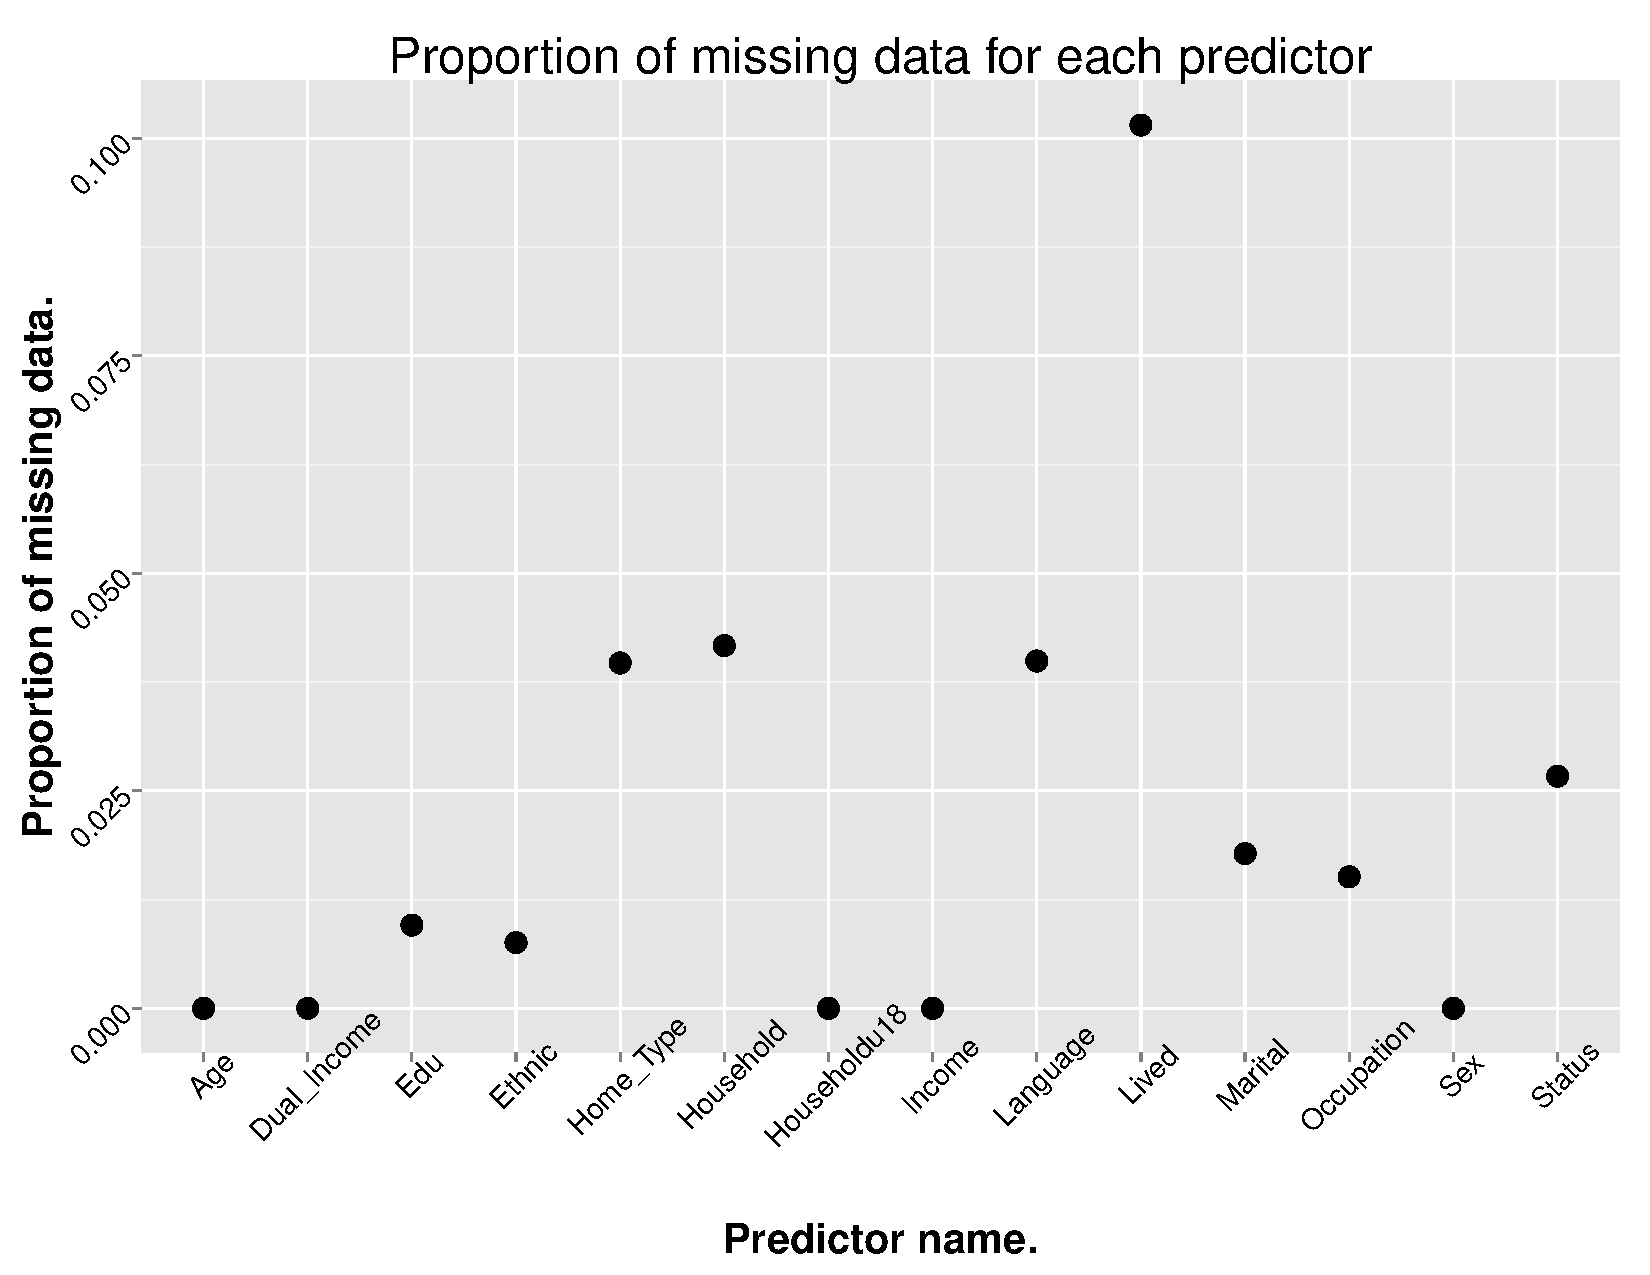
\includegraphics[width=1.0\textwidth]{HandlingMissingData/PropMissingData.pdf}
  \caption{Proportion of Missing Data.}
  \label{Proportion}
\end{figure}


\section{Frequ}
\section{Bayesian Analysis}
We used RJAGS in our Bayesian analysis. RJAGS is a way of calling JAGS from with in \textsf{R}. JAGS is a program for the statistical analysis of Bayesian models by Markov Chain Monte Carlo, MCMC. MCMC is a way of sampling form a distribution by using a Markov chain with its equilibrium distribution the same as the distribution we wish to sample from. A MCMC has two stages a burn in stage, where the Markov chain hasn't reached equilibrium, and a converged stange, where the chain has reached equilibrium.
\\\\
When using \textsf{R} it calls $\beta_0$ beta[1].
\subsection{Saturated Model}
We start the Bayesian analysis by modelling the saturated model with the missing data handled by just simply omitting it, later on we use the mice method mentioned earlier to handle the missing values. We have chosen to use a vague prior on each of our parameters, $\beta_i$, and for the precision, $\tau$. The model string  for this is 
\begin{verbatim}
modelstring = "
model {
for (i in 1:n) {
mean[i] =  inprod(X[i,],beta)
y[i]~dnorm(mean[i],tau)
}
for (j in 1:p) {
beta[j]~dnorm(0,0.001)
}
tau~dgamma(1,0.001)
}
"
\end{verbatim}
The MCMC had a burn in of 1000 iterations and a run of 10,000 iterations. From the plots of $\beta_1$ to $\beta_4$ we can see that the distribution converged. This is shown in Figure~\ref{saturated_beta1-4} by the "furry caterpillar" effect we see.
\begin{figure}[h!]
\centering
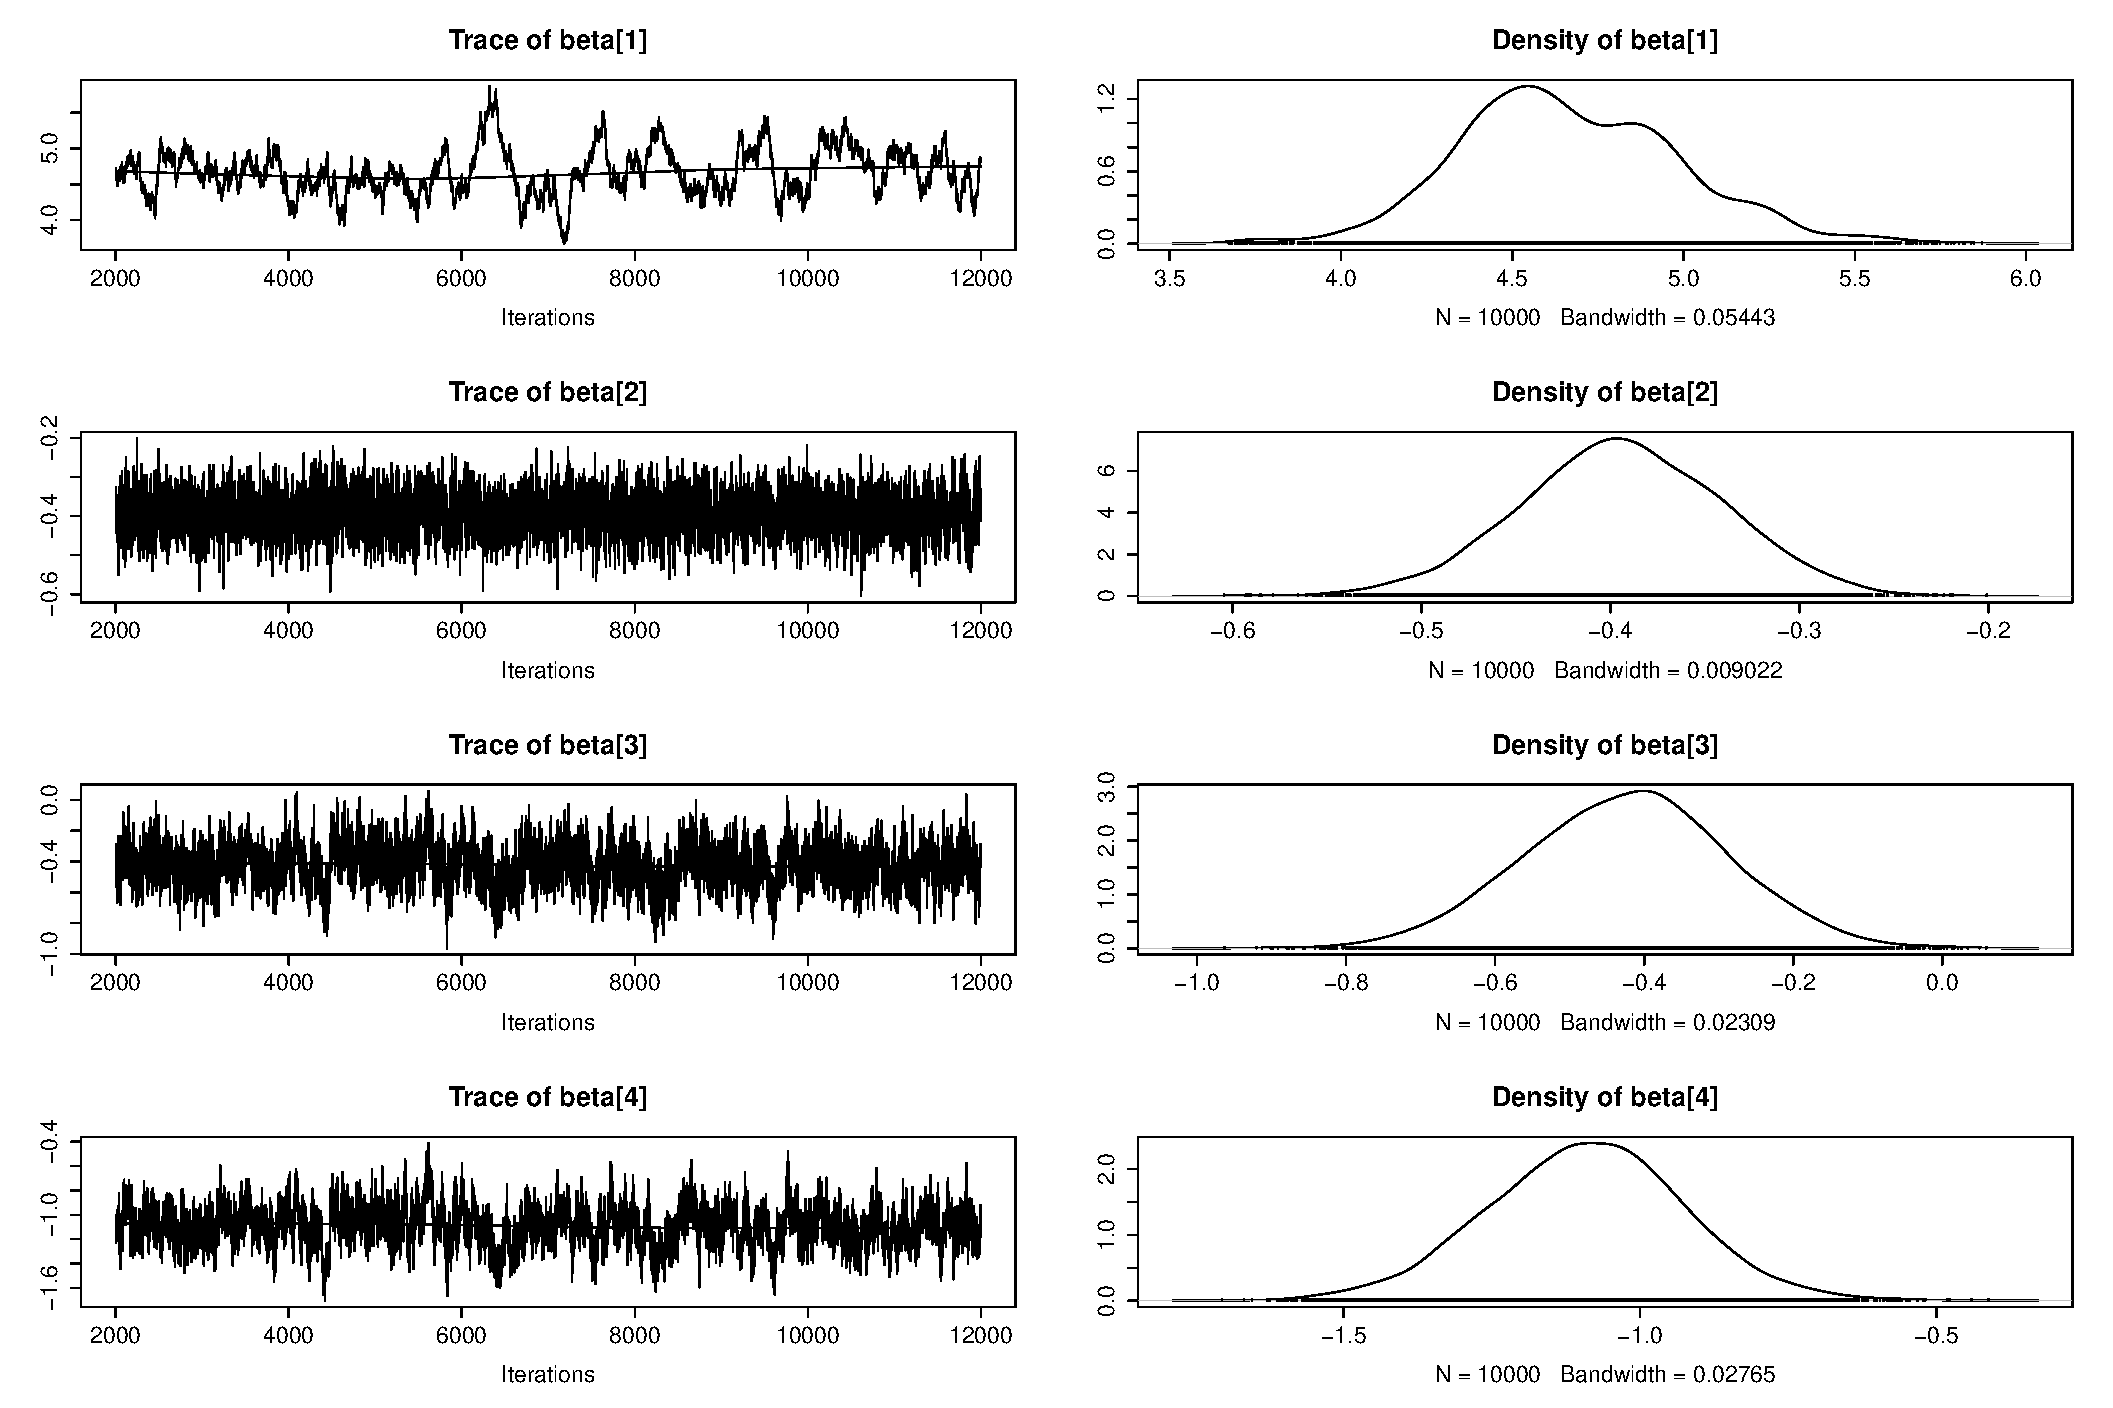
\includegraphics[width = 0.9\textwidth]{saturatedOutput/beta1-4.pdf}
\caption{Trace and density plots for the parameters $\beta_0, \beta_1, \beta_2$ and $\beta_3$.}
\label{saturated_beta1-4}
\end{figure}
\subsection{Model with Variable Selection}
The model can be improved upon by using a model that does variable selection and random effects with prior inclusion. This means that the model will no longer have all the variables which will give us a model which is less likely to over fit and will have less bias. The random effects means that the variable value is now changed with a variable probability where the probability comes from a normal distribution. The model string we used to incorporate this is
\begin{verbatim}
modelstring = "
model{
for(i in 1:n){
mean[i] = inprod(X[i,], beta)
y[i] ~ dnorm(mean[i],tau)
}
for (j in 1:p) {
ind[j] ~ dbern(pind)
betaT[j] ~ dnorm(0,taub)
beta[j] = ind[j]*betaT[j]
}
tau ~ dgamma(1, 0.001)
taub ~ dgamma(1, 0.001)
pind ~ dbeta(2,8)
}
"
\end{verbatim}
\begin{figure}[H]
\centering
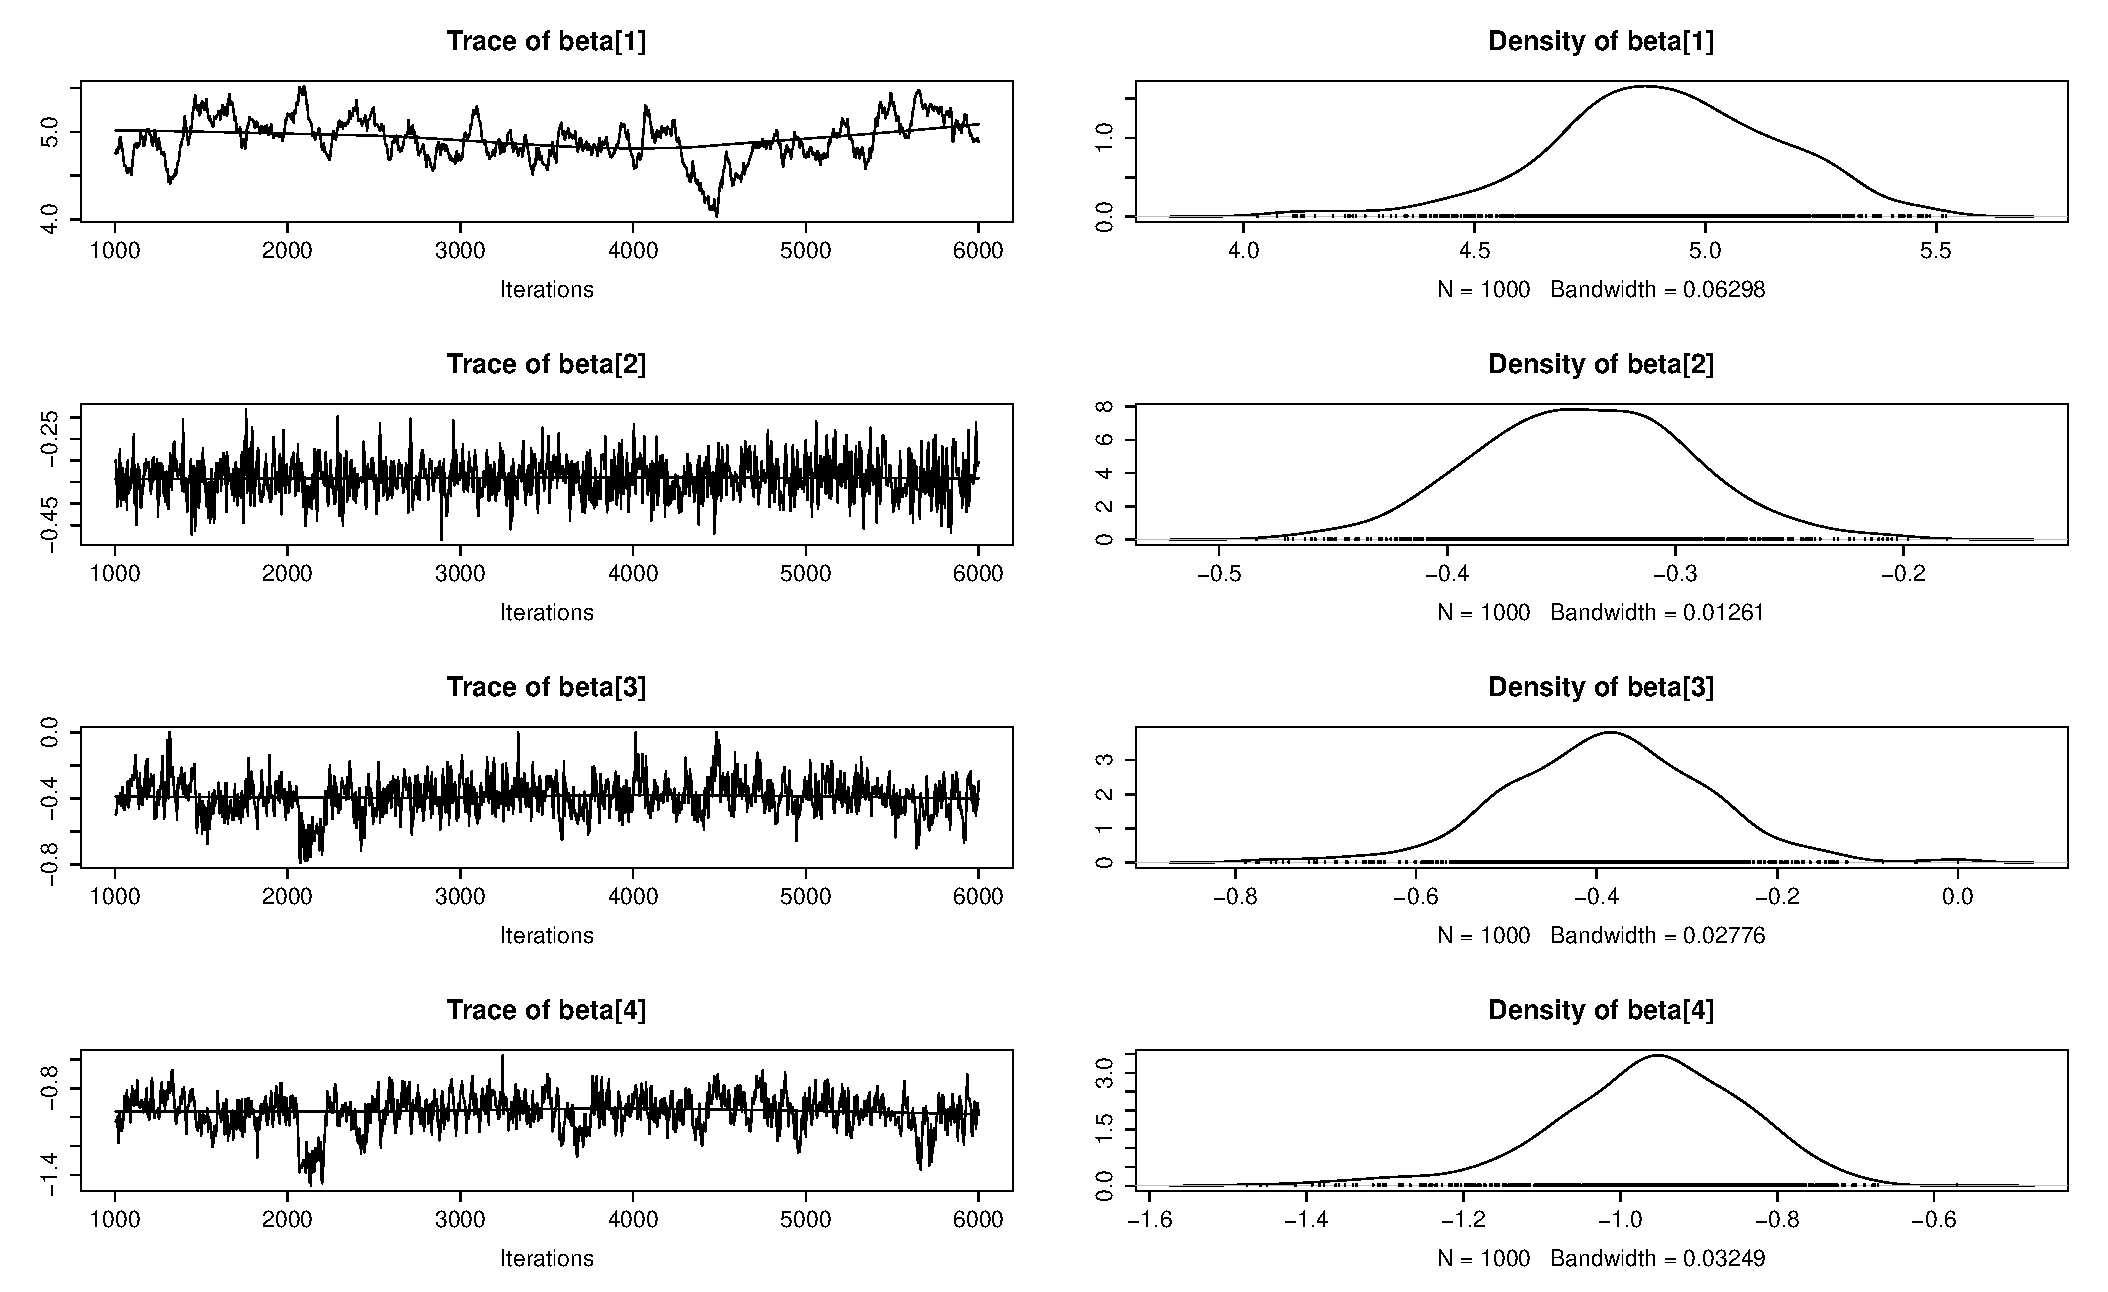
\includegraphics[width = 0.9\textwidth]{micePlot.pdf}
\caption{Trace and density plots for $\beta_0, \beta_1, \beta_2$ and $\beta_3$}
\label{micePlot}
\end{figure}
We used this model to the data where the missing values had been replaced using the MICE method mention in Section~\ref{handling}. Since this is a better approach to modelling the data we ran the MCMC for a longer period of time. The burn is period is 1000 iterations and the run is 5000 iterations. As you can see in Figure~\ref{micePlot} the trace plot is now not as condensed because the JAGS model has included variable selection so some iterations give a value of 0. Figure~\ref{notIncluded} shows that the model has chosen for $\beta_{20}, \beta_{21}, \beta_{22}$ and $\beta_{23}$ to not be included in the model. This is shown by the trace plot regularly being 0 and in the density plots. The density plot for $\beta_21$ and $\beta_22$ are represented by histograms are there are so few values which are not approximately 0.
\begin{figure}[H]
\centering
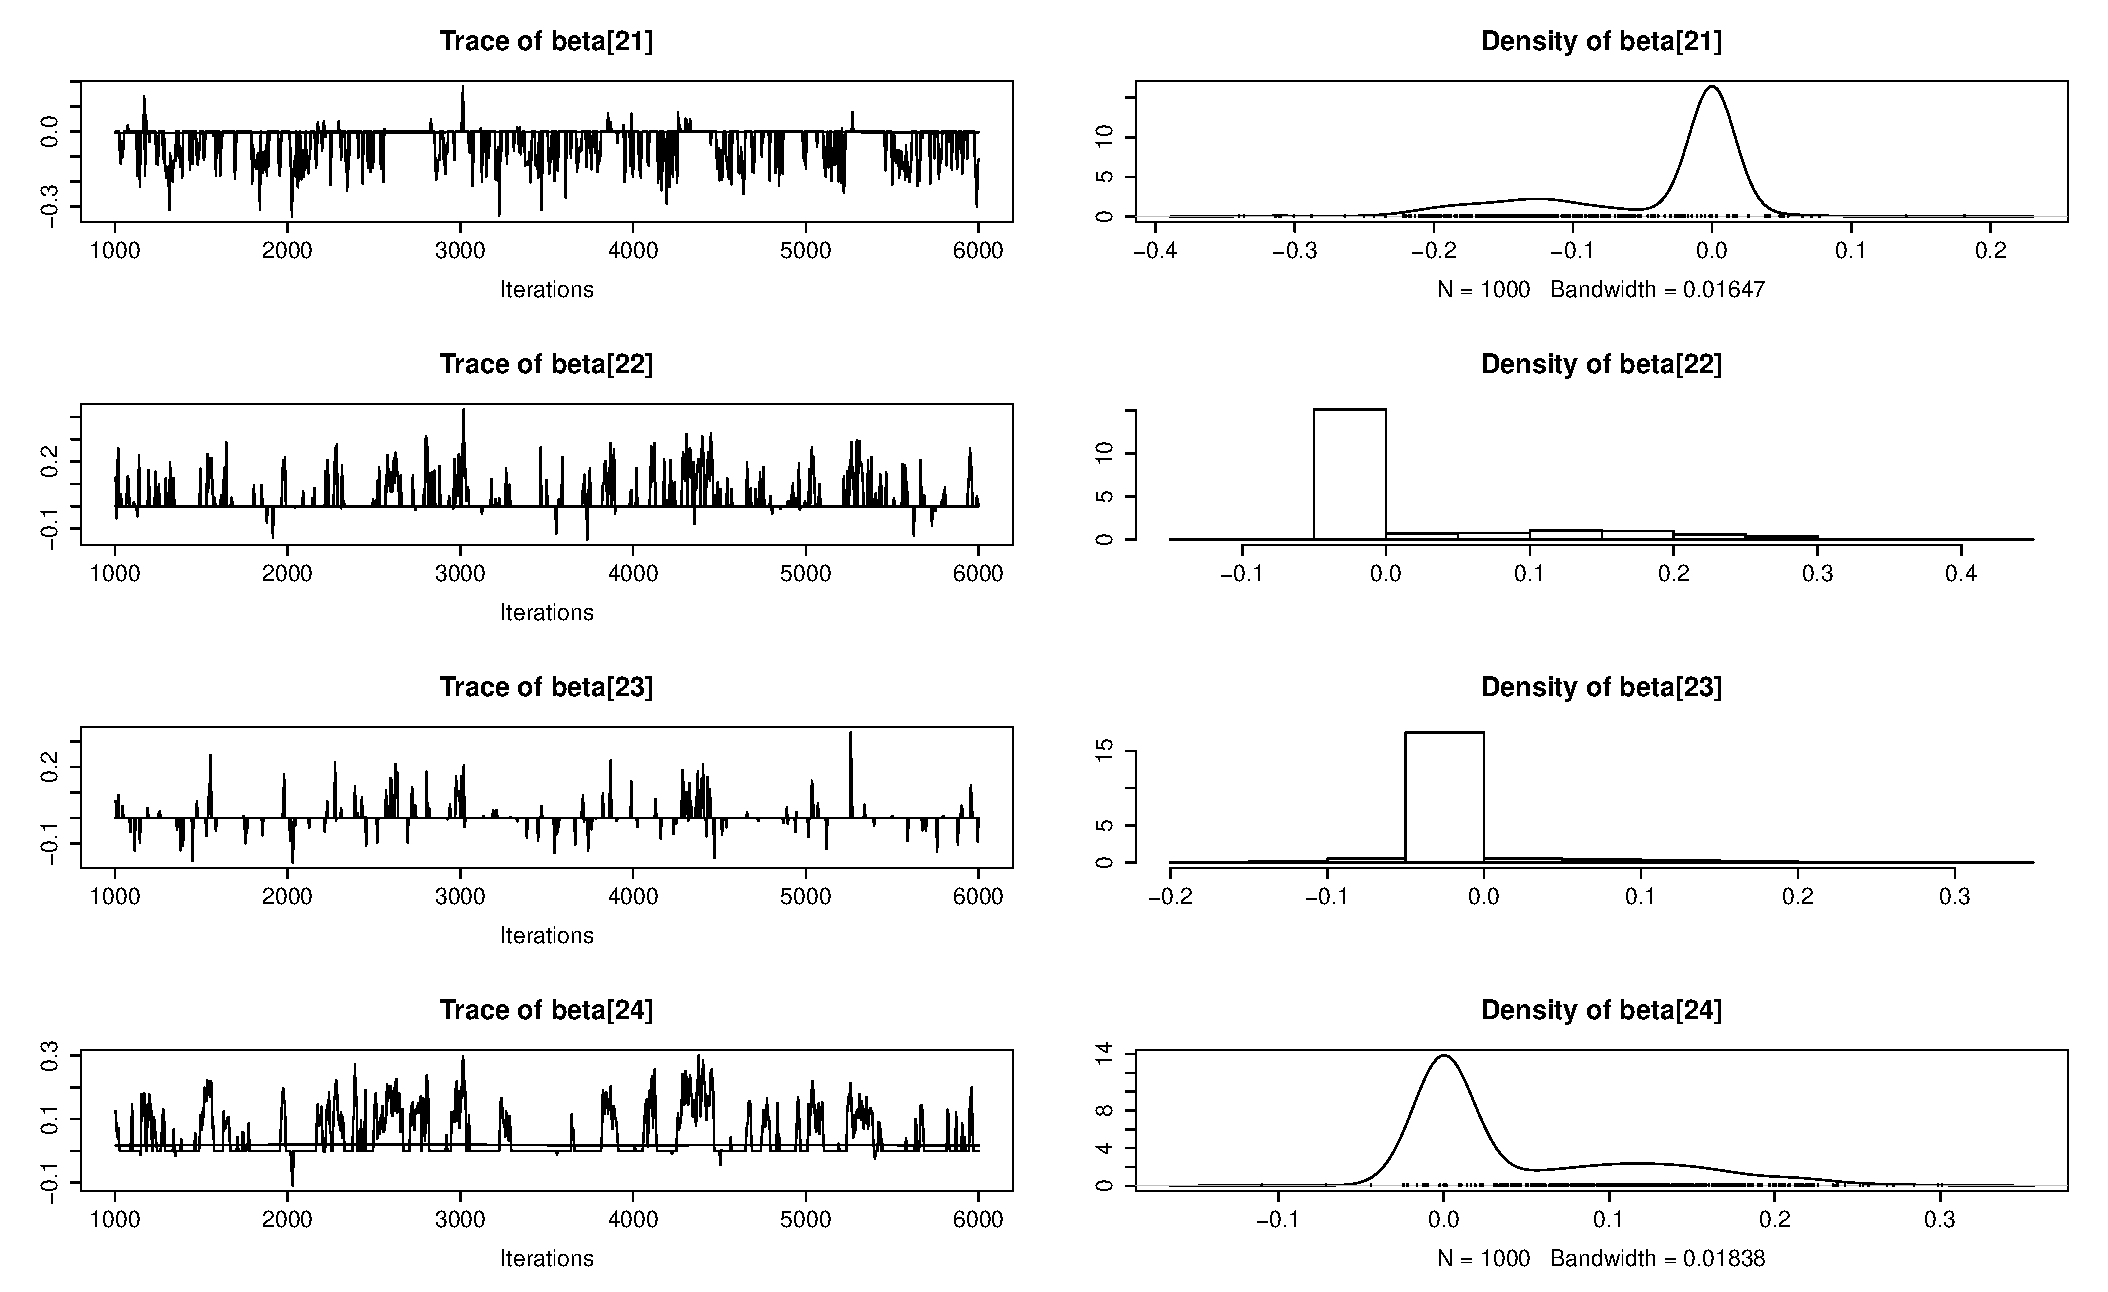
\includegraphics[width = 0.9\textwidth]{notIncludedBetas.pdf}
\caption{}
\label{notIncluded}
\end{figure}
\noindent The variable selection process has included some of the predictors. The \textsf{ind} vector can be though of as the probability that the corresponding predictor is in the model. Below we have the \textsf{R} output showing the \textsf{ind} values. We can see here that \textsf{ind[21] - ind[28]}, for example, have some uncertainty whether there respective variables should be in the model. The value for \textsf{ind[28]} has the lowest mean value and therefore the variable it corresponds to, \textsf{Householdu18}, is least likely to be in the model. 
\\\\
It is worth noticing that the variables \textsf{ind[21] - ind[28]}, representing Lived[2] - Lived[5], are potentially as low as they are because $10\%$ of the data corresponding to this, which is how long a person had lived in their house, was initially missing and therefore had be created during the MICE method.
{\small
\begin{verbatim}
              Mean       SD  Naive SE Time-series SE
ind[1]    1.000000 0.000000 0.0000000      0.0000000
ind[2]    1.000000 0.000000 0.0000000      0.0000000
ind[3]    0.994000 0.077266 0.0024434      0.0030262
ind[4]    1.000000 0.000000 0.0000000      0.0000000
ind[5]    1.000000 0.000000 0.0000000      0.0000000
ind[6]    1.000000 0.000000 0.0000000      0.0000000
ind[7]    1.000000 0.000000 0.0000000      0.0000000
ind[8]    0.990000 0.099549 0.0031480      0.0068224
ind[9]    1.000000 0.000000 0.0000000      0.0000000
ind[10]   1.000000 0.000000 0.0000000      0.0000000
ind[11]   1.000000 0.000000 0.0000000      0.0000000
ind[12]   1.000000 0.000000 0.0000000      0.0000000
ind[13]   1.000000 0.000000 0.0000000      0.0000000
ind[14]   1.000000 0.000000 0.0000000      0.0000000
ind[15]   1.000000 0.000000 0.0000000      0.0000000
ind[16]   1.000000 0.000000 0.0000000      0.0000000
ind[17]   1.000000 0.000000 0.0000000      0.0000000
ind[18]   1.000000 0.000000 0.0000000      0.0000000
ind[19]   1.000000 0.000000 0.0000000      0.0000000
ind[20]   1.000000 0.000000 0.0000000      0.0000000
ind[21]   0.339000 0.473607 0.0149768      0.0333299
ind[22]   0.254000 0.435515 0.0137722      0.0292305
ind[23]   0.148000 0.355278 0.0112349      0.0134316
ind[24]   0.379000 0.485381 0.0153491      0.0457288
ind[25]   0.972000 0.165055 0.0052195      0.0234233
ind[26]   0.259000 0.438305 0.0138604      0.0341916
ind[27]   0.564000 0.496135 0.0156892      0.1392019
ind[28]   0.166000 0.372267 0.0117721      0.0408814
ind[29]   1.000000 0.000000 0.0000000      0.0000000
ind[30]   1.000000 0.000000 0.0000000      0.0000000
ind[31]   0.660000 0.473946 0.0149875      0.0249466
ind[32]   1.000000 0.000000 0.0000000      0.0000000
ind[33]   1.000000 0.000000 0.0000000      0.0000000
ind[34]   1.000000 0.000000 0.0000000      0.0000000
ind[35]   0.297000 0.457165 0.0144568      0.0389590
ind[36]   0.184000 0.387678 0.0122595      0.0354303
ind[37]   0.857000 0.350248 0.0110758      0.0114945
ind[38]   0.698000 0.459355 0.0145261      0.0402731
ind[39]   0.318000 0.465932 0.0147341      0.0258775
ind[40]   0.254000 0.435515 0.0137722      0.0405610
ind[41]   0.221000 0.415128 0.0131275      0.0309514
ind[42]   0.988000 0.108940 0.0034450      0.0074873
ind[43]   0.167000 0.373162 0.0118004      0.0123641
\end{verbatim}}


\end{document}